% This file was created with tikzplotlib v0.10.1.
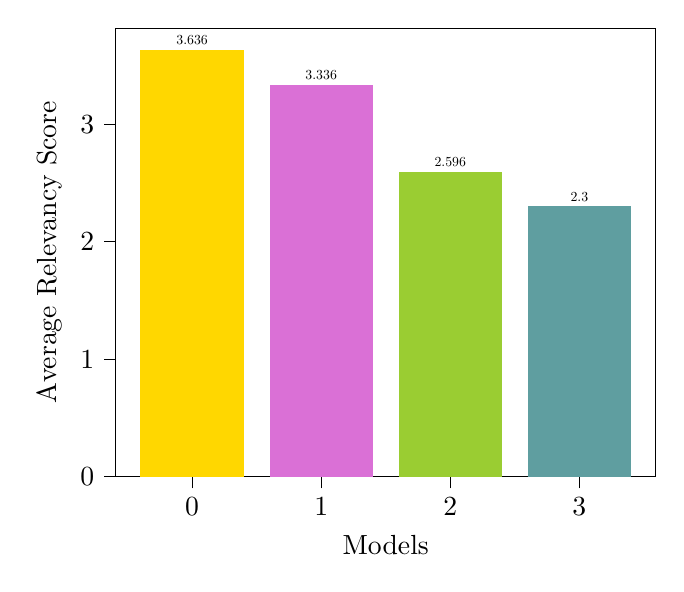
\begin{tikzpicture}

\definecolor{cadetblue}{RGB}{95,158,160}
\definecolor{darkgray176}{RGB}{176,176,176}
\definecolor{gold}{RGB}{255,215,0}
\definecolor{orchid}{RGB}{218,112,214}
\definecolor{yellowgreen}{RGB}{154,205,50}

\begin{axis}[
tick align=outside,
tick pos=left,
x grid style={darkgray176},
xlabel={Models},
xmin=-0.59, xmax=3.59,
xtick style={color=black},
y grid style={darkgray176},
ylabel={Average Relevancy Score},
ymin=0, ymax=3.8178,
ytick style={color=black}
]
\draw[draw=none,fill=gold] (axis cs:-0.4,0) rectangle (axis cs:0.4,3.636);
\draw[draw=none,fill=orchid] (axis cs:0.6,0) rectangle (axis cs:1.4,3.336);
\draw[draw=none,fill=yellowgreen] (axis cs:1.6,0) rectangle (axis cs:2.4,2.596);
\draw[draw=none,fill=cadetblue] (axis cs:2.6,0) rectangle (axis cs:3.4,2.3);
\draw (axis cs:0,3.636) ++(0pt,0pt) node[
  scale=0.5,
  anchor=south,
  text=black,
  rotate=0.0
]{3.636};
\draw (axis cs:1,3.336) ++(0pt,0pt) node[
  scale=0.5,
  anchor=south,
  text=black,
  rotate=0.0
]{3.336};
\draw (axis cs:2,2.596) ++(0pt,0pt) node[
  scale=0.5,
  anchor=south,
  text=black,
  rotate=0.0
]{2.596};
\draw (axis cs:3,2.3) ++(0pt,0pt) node[
  scale=0.5,
  anchor=south,
  text=black,
  rotate=0.0
]{2.3};
\end{axis}

\end{tikzpicture}
